\dev{Emile Martinez}{}

\textit{Mettre une description}

\paragraph{Problème} On a des exemples $E = \{(x, c) \in X\times Y\}$ et on a $x \in X$ dont on cherche sa classe.\\
Ici $X = \mathbb R^d$

\begin{com}
	Ici on parle de $Y$, mais c'est une liste de classes.
\end{com}

\paragraph{Paramètre} $k > 0$ un entier

\begin{algo} Algorithme des $k$-plus proche voisins
	\begin{enumerate}
		\item On cherche les k plus proches voisins de $x$ dans $T$
		\item On renvoie la classe majoritaire parmi ces $k$ classes
	\end{enumerate}
\end{algo}

\begin{example}
	Imaginons qu'on ait un capteur permettant de détecter le poids d'un animal qui passe et sa taille. Comment savoir quel animal était-ce ?\\ \centering
	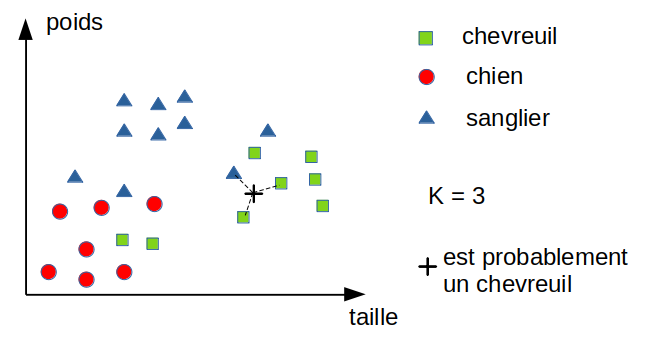
\includegraphics[scale=0.4]{Developpements/k voisins/graphe.png}
\end{example}

\paragraph{Question} Quel choisir k ?

\begin{com}
	Si $k$ est trop petit.
\end{com}
\begin{center}
	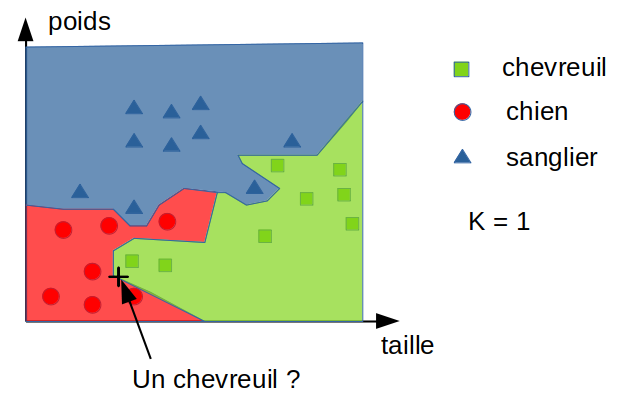
\includegraphics[scale=0.4]{Developpements/k voisins/graphe2.png}
\end{center}

$\to$ On a une trop grande influence des cas particuliers $\to$ sur apprentissage.

Exemple classique de sur apprentissage quand on veut approximer des points par une courbe : \\
\begin{minipage}{0.5\linewidth}
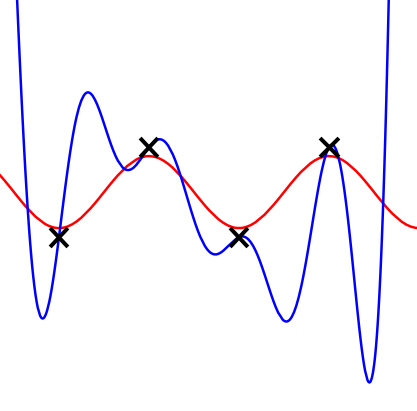
\includegraphics[scale=0.4]{Developpements/k voisins/sur_apprentissage.png}
\end{minipage}\begin{minipage}{0.5\linewidth}
La ligne bleue colle mieux aux données mais à l'air moins bien que la rouge.
\end{minipage}

\paragraph{Influence lointaine} Si $K$ est choisi trop grand, des points trop loin auront une trop grande influence.
\begin{center}
	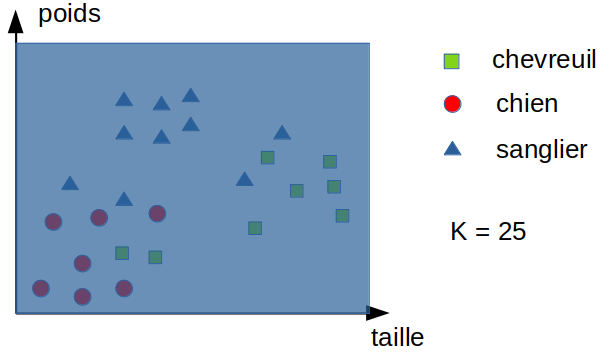
\includegraphics[scale=0.4]{Developpements/k voisins/graphe3.png}	
\end{center}

\begin{com}
	Super il faut le choisir bien, mais ca nous dit pas comment. 
\end{com}

\paragraph{Comment le choisir ?} On en essaie plein.\\
On sépare $E$ en $D_A$ et $D_T$ (avec $\dfrac{\left| D_A \right|}{|E|} \simeq 80\%$). On essaye alors de prédire $D_T$ en utilisant $D_A$ et on regarde pour quel $k$ on a la meilleur performance.

\paragraph{Question} Pourquoi séparer ?\\
$\to$ Car si on faisait sur les mêmes éléments, on éviterait pas le biais du surapprentissage.
\begin{com}
	Ici revenir sur l'exemple pour le montrer. En disant que avec $k =1$ on aurait $100\%$ de réussite.
\end{com}

\paragraph{Validation croisée} Si on a pas assez de données ?
\begin{com}
	Chaque donnée joue alternativement le rôle de données de test et de données d'entrainement.
\end{com}
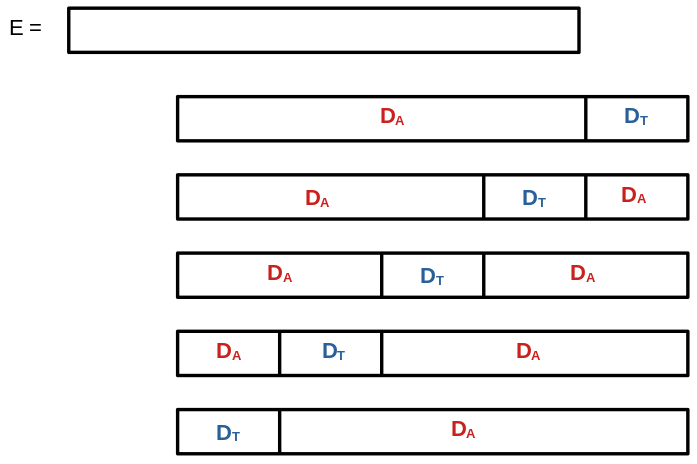
\includegraphics[scale=0.4]{Developpements/k voisins/validation_croisee.png}


\paragraph{Complexité} Comment chercher les $K$ plus proches voisins parmi $N$ points ?
	\begin{itemize}[label=$\bullet$]
		\item En cherchant pour $i$ allant de $1$ à $K$ le point le plus proche puis en l'enlevant.
			\\ $\to O(N\times K)$ 
		\item En parcourant les $N$ points et en gardant à chaque fois les $K$ plus proches (quand on en trouve un plus petit, on enlève le plus loin parmi les $K$).
			\\ $\to O(N \times \log K)$ si on utilise les structures de données adéquates
		\item En faisant des pré-calculs, on peut obtenir une structure permettant de faire la recherche des $K$ plus proche voisins en $O(\log N + K)$ en moyenne. $\to$ rentable pour beaucoup de recherche.
		\begin{com}
			Faire l'analogie avec la dimension $1$ et les listes triées.
		\end{com}
	\end{itemize}

\paragraph{Notion de distance} On utilise ici la distance euclidienne mais on pourrait également utiliser d'autres distances, comme la distance de Manhattan.

\paragraph{Normalisation des paramètres} Il se peut qu'une coordonnée soit beaucoup plus grande que toutes les autres et ait beaucoup trop d'importances. Et même, quand on compare des grandeurs différentes, comment choisir l'unité que l'on prend (influençant le poids de cette grandeur)

\begin{center}
	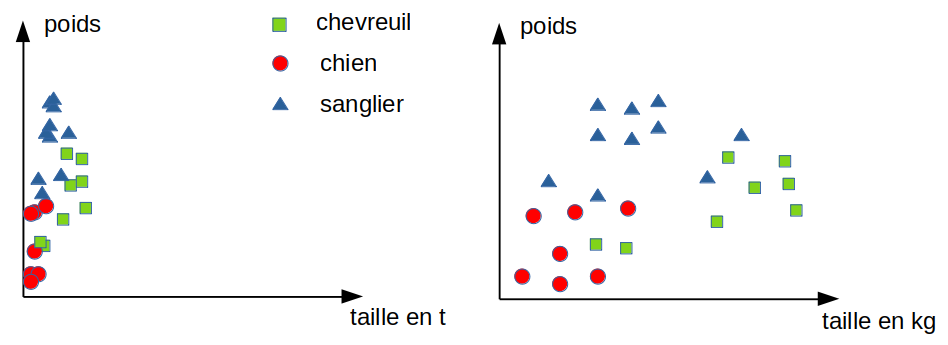
\includegraphics[scale=0.5]{Developpements/k voisins/decale.png}
\end{center}


